\documentclass[9pt]{article}
\usepackage[a4paper,margin=1in]{geometry}
\usepackage{times}
\usepackage{tikz}
\usetikzlibrary{positioning}
\parindent=0pt
\begin{document}
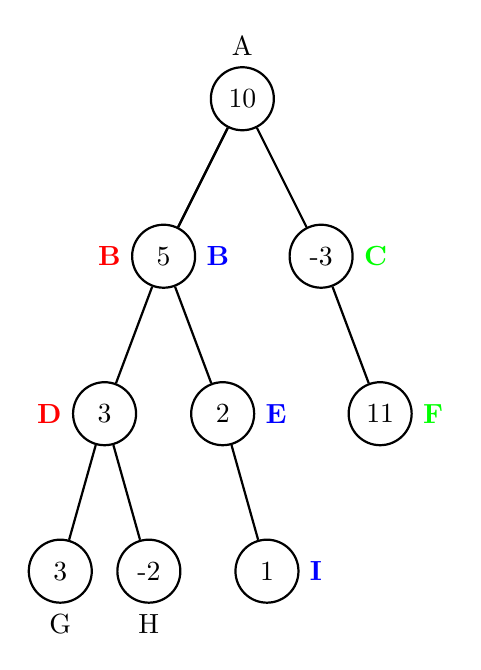
\begin{tikzpicture}[mnode/.style={draw=black,circle,inner sep=2pt,minimum size=8mm},thick]
  \node[mnode] (A) at (0,0) {10};
  \node[mnode] (B) at (-1,-2) {5};
  \node[mnode] (C) at (1, -2) {-3};
  \node[mnode] (D) at (-1.75, -4) {3};
  \node[mnode] (E) at (-0.25, -4) {2};
  \node[mnode] (F) at (1.75, -4) {11};
  \node[mnode] (G) at (-2.3125, -6) {3};
  \node[mnode] (H) at (-1.1875,-6) {-2};
  \node[mnode] (I) at (.3125,-6) {1};
  \node[above] at (A.north) {A};
  \node[left,color=red] at (B.west) {\textbf{B}};
  \node[right,color=blue] at (B.east) {\textbf{B}};
  \node[right,color=green] at (C.east) {\textbf{C}};
  \node[left,color=red] at (D.west) {\textbf{D}};
  \node[right,color=blue] at (E.east) {\textbf{E}};
  \node[right,color=green] at (F.east) {\textbf{F}};
  \node[below] at (G.south) {G};
  \node[below] at (H.south) {H};
  \node[right,color=blue] at (I.east) {\textbf{I}};
  \begin{scope}[-]
    \draw (A) -- (B);
    \draw (A) -- (C);
    \draw (D) -- (B);
    \draw (E) -- (B);
    \draw (C) -- (F);
    \draw (G) -- (D);
    \draw (H) -- (D);
    \draw (I) -- (E);
    \draw (A) -- (B);
  \end{scope}
\end{tikzpicture}

\vspace{0.2in}
As highlighted in the picture, the solution is very general. It can
\begin{itemize}
  \item begin at any node,
  \item a node may be part of multiple paths,
  \item the tree may contain negative nodes so you may never discard a node
        just because it's value is larger than targetSum.
\end{itemize}

Thus, it's very apparent the solution must traverse the full tree, and multiple
times for all possible cases. Let's try to divide the solution. The solution
\begin{itemize}
  \item can be sub-divided to solutions just in the left and right sub-trees,
  \item and solutions in left and right sub-trees including the current node.
  \item The total of these gives the final answer.
\end{itemize}

Let $\Pi(n, t)$ be short for pathSum(node, targetSum), and let $n.l$ and $n.r$
represent node.left and node.right, and let $n.v$ represent node.value. Let $\pi(n,t)$ is the number of paths starting from $n$ with target sum $t$.
So, a general strategy is that the solution $\Pi(n, t)$ is recursively
\begin{equation}
  \Pi(n, t) = \Pi(n.l, t) + \Pi(n.r, t) + \pi(n.l, t-n.v) + \pi(n.r, t-n.v)
\end{equation}
where, the first two terms count number of paths in either sub-trees that sum to
$t$ without including the current node, while the latter two terms include the
current node in the target sum. This equation makes sense since each of the terms
are mutually exclusive. So, they can be summed up.

Edge cases?
Say in the figure below the \textcolor{blue}{\textbf{B-E-I}} path, there was a long list of nodes
with alternative +1, -1. How many nodes down a path must one go? Do they all
count as their own unique paths? This algo will enumerate them all, but the
worst case complexity would be poor. I don't see any opportunity to memoize or
DP-ize the solution either. Maybe a bottom-up solution?
\end{document}
